\chapter{Referencial Teórico}

\index{Referencial Teórico }
	 
% \section{Fundamentos Teóricos}
\par
    Para melhor compreensão do conteúdo apresentado neste trabalho, este capítulo tem como objetivo explicar os fundamentos conceituais necessários para garantir a boa compreensão e evolução do conteúdo.
    
\section{Redes}

\subsection{Grafos}
Grafos são formas de estruturação de dados ligados pertencentes ao mesmo conjunto. Um elemento recebe a denominação de nó ou vértice. As relações entre os nós são definidas por \textit{arestas}.
Para exemplificação, tome como nós, cidades \textit{n1},\textit{n2}, \textit{n3} e \textit{n4}, onde as estradas que fazem conexão entre estas cidades representam as arestas \ref{graph_base}. Com este conceito, pode-se modelar estas ligações em forma de grafo. \cite{Graph_teory}
%
%Imagem
\begin{figure}[ht!]
\centering
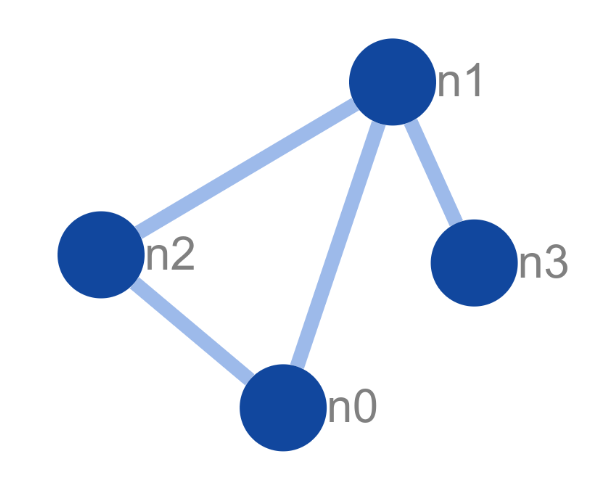
\includegraphics[width=50mm]{Images/graph_base.png}
\caption {Representação em grafo
\label{graph_base}}
\flushleft{Fonte: Produzido pelos autores.}
\end{figure}


\subsection{Grafos com pesos}
São grafos que possuem um \textbf{grau de importância} (também chamado de peso) em cada \textbf{aresta}, este \textbf{grau de importância} tem significado apenas em nível de abstração, ou seja, não carrega uma interpretação predefinida. Geralmente, exprime o quão \textbf{relacionado} um nó está com outro, onde esta informação é interpretada de acordo com o contexto no qual está inserido.\cite{Graph_teory}

Figura representativa~\ref{graph_wheigth}.
%
%Imagem
\begin{figure}[ht!]
\centering
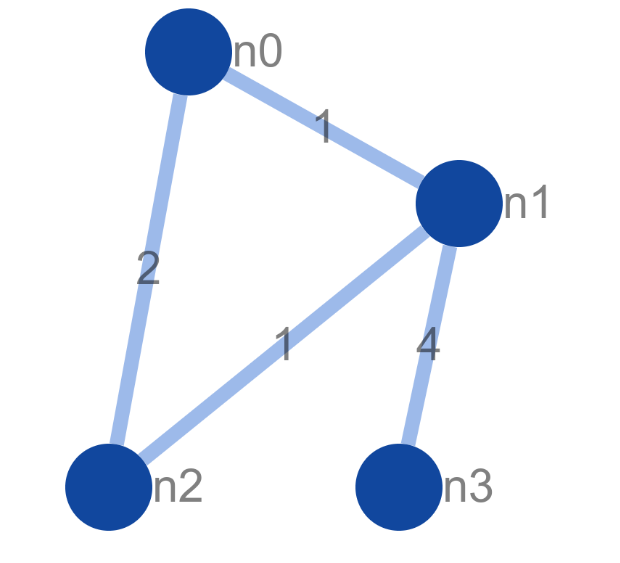
\includegraphics[width=50mm]{Images/graph_wheigth.png}
\caption {Grafo com peso
\label{graph_wheigth}}
\flushleft{Fonte: Produzido pelos autores.}
\end{figure}

\subsection{Passeio}
É uma sequência específica de nós ligados, partindo de \textbf{\textit{p}} e chegando em \textbf{\textit{g}} \cite{Pavlopoulos2011}. Onde o \textbf{comprimento} do \textit{passeio} é determinado pelo número de \textit{arestas} percorridas.
%
Tomando o \textsl{grafo} representado pela Figura~\ref{graph_path}, um dos \textbf{passeios} possíveis de \textsl{p} a \textsl{q} é o conjunto \textsl{A}, formado pelos nós visitados \textit{A =\{p,r,t,v,t,q\}}. O \textbf{comprimento do passeio} \textsl{A} é \textit{6}, como também pode ser definido como o tamanho do \textit{conjunto} de nós visitados \textit{menos 1}.
%
%Imagem
\begin{figure}[ht!]
\centering
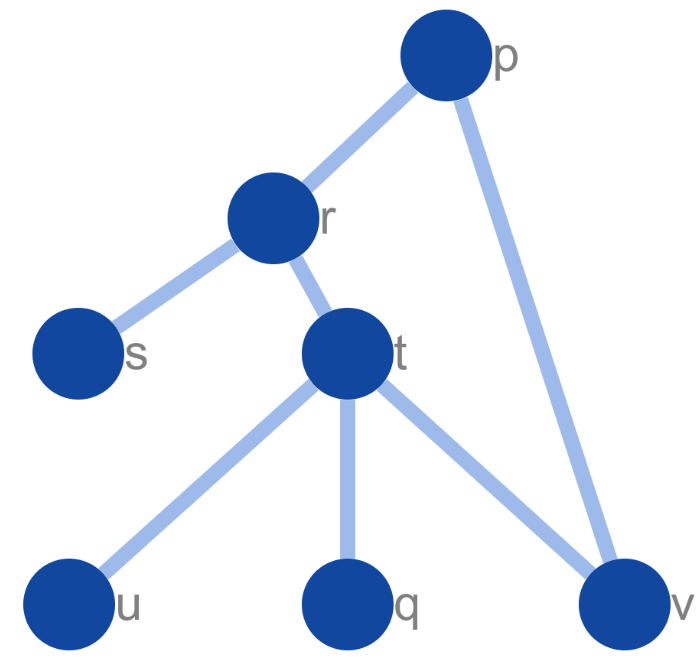
\includegraphics[width=50mm]{Images/graph_path.png}
\caption {Grafo
\label{graph_path}}
\flushleft{Fonte: Produzido pelos autores.}
\end{figure}


\subsection{Caminho e distância}
Assim como o \textit{passeio}, o \textit{caminho} é uma sequência específica de nós ligados. Porém este não possui vértices repetidos, ou seja, não passa duas vezes pelo mesmo vértice \cite{Pavlopoulos2011}. 
Se tomarmos como exemplo o grafo da imagem \ref{graph_path}, um \textbf{caminho} de \textit{p} a \textit{q} é a sequencia de nós \textit{\{p,r,t,q\}}. 
A \textbf{distância} do \textit{caminho} é definida pela soma dos pesos em suas arestas em \textit{grafos com pesos}. Para os \textit{grafos sem peso}, a \textbf{distância} é definida pela quantidade de arestas presentes no \textit{caminho}, implicitamente definindo o peso de cada \textit{aresta} como \textit{1} e executando a soma das mesmas.
No \textbf{caminho} \textit{\{p,r,t,q\}} a \textbf{distância} entre \textit{p} e \textit{q} é \textit{4}.


%\subsection{Distância}
%Em grafos com peso, é definida pela soma dos pesos das arestas em um determinado caminho.
%Em grafos sem peso, é definida como a quantidade de arestas (aresta peso 1) em um determinado %caminho.

%Imagem


\subsection{Hub}
Hub é um nó que possui muitas arestas, ou seja, um nó que se liga a muitos outros nós \cite{Pavlopoulos2011}.
Na imagem \ref{graph_hub} o \textsl{hub} é o nó \textsl{t}, ou seja, é o nó que possui mais arestas \textsl{6} do grafo.
%
%Imagem - HUB
\begin{figure}[ht!]
\centering
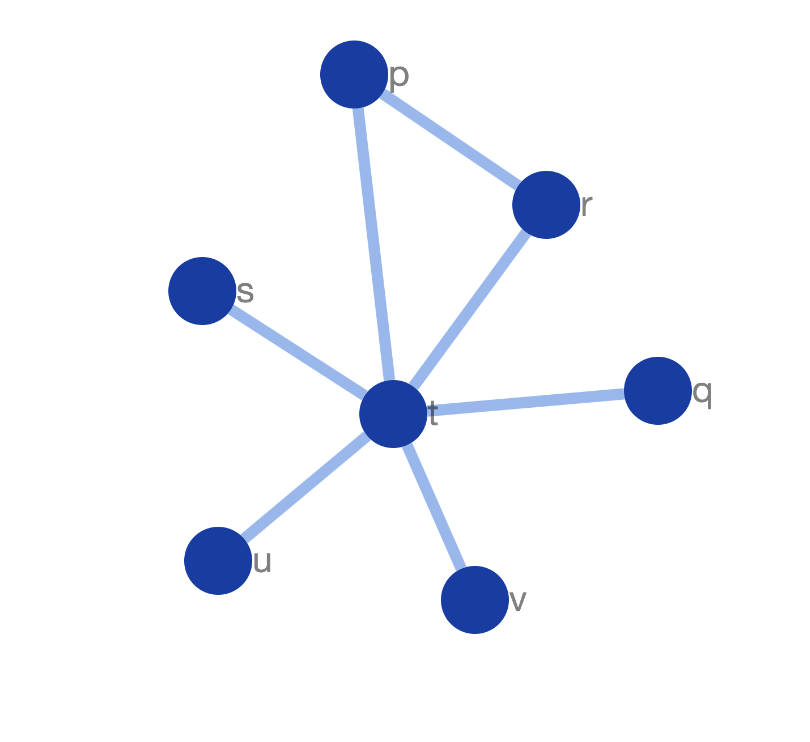
\includegraphics[width=80mm]{Images/graph_hub.png}
\caption {Representação de \textsl{Hub}
\label{graph_hub}}
\flushleft{Fonte: Produzido pelos autores.}
\end{figure}


\subsection{Bridge}
O quão ponte o nó é em relação a dois ou mais \textsl{Hubs}, ou seja, é uma medida que determina o quanto um nó liga dois grandes agrupamentos \cite{Hwang2006}. Na Figura~\ref{graph_bridge} o nó \textbf{\textsl{n16}} é um definido como bridge e os nós \textbf{\textsl{t}} e \textbf{\textsl{n13}} são \textsl{Hubs}, mesmo o nó \textsl{\textbf{n16}} não estando diretamente ligado nos nós \textsl{Hubs}, ele apresenta o comportamento de \textsl{Bridge} por estar conectando os dois grandes agrupamentos.
%
%Imagem - BRIGDE
\begin{figure}[ht!]
\centering
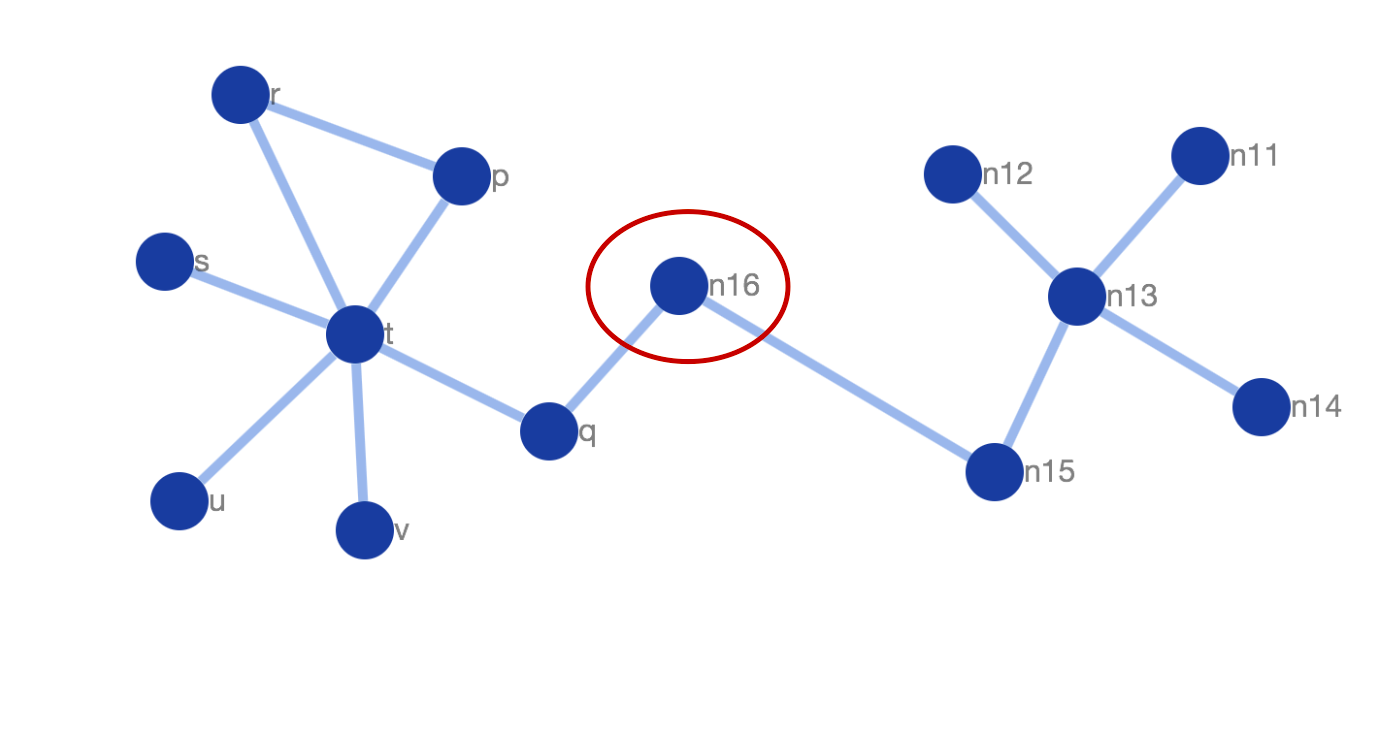
\includegraphics[width=\textwidth]{Images/graph_bridge.png}
\caption {Representação de um nó \textsl{bridge}
\label{graph_bridge}}
\flushleft{Fonte: Produzido pelos autores.}
\end{figure}

\subsection{Menor caminho ou caminho mínimo}
Quando se trata de grafos o \textbf{caminho mínimo} é aquele que possui a menor distância entre dois nós (\textsl{p} e \textsl{g}) \cite{Dijkstra1959}. No grafo com pesos representado pela Figura~\ref{graph_wheigth}, o caminho mínimo entre os nós \textsl{n2} e \textsl{n3} é dado pelo conjunto de nós \textsl{\{n2,n1,n3\}}, sendo a distância entre \textsl{n2} e \textsl{n3} igual a \textsl{5}. Um outro caminho válido mas que não é mínimo entre \textsl{n2} e \textsl{n3} é dado pelo conjunto de nós conectados \textsl{\{n2,n0,n1,n3\}}, no qual a distância entre \textsl{n2} e \textsl{n3} é igual a \textsl{7}. Ambos são caminhos válidos no mesmo grafo, porém o menor caminho possível entre \textsl{n2} e \textsl{n3} neste grafo é \textsl{\{n2,n1,n3\}}.
%Imagem

\subsection{Redes complexas}
Redes são formas de representação de dados ligados. Partindo deste princípio, as redes complexas correspondem a grafos, de forma que representem e adotem os conceitos utilizados na \textsl{Teoria de Grafos}. Este conceito foi muito importante para representação de sistemas complexos, sendo que os mesmos podem ser representados em forma de grafos e consequentemente em rede \cite{Strogatz2001}. Porém, redes complexas devem apresentar estruturas topológicas não triviais, ou seja, possuírem um conjunto de vértices que sejam interconectados por arestas \cite{Barabasi2003}.
%

O estudo de dados ligados tendo como a representação de intensidade e o sentido de suas conexões, faz com que muitos problemas do mundo real possam ser apresentados em redes complexas através de analogias. Esta possibilidade de representação, faz com que um problema aparentemente indescritível, seja modelado e representado por uma rede complexa, podendo assim ser estudado utilizando os ferramentais desenvolvidos para grafos e redes complexas. Isto auxilia a resolução do problema, em vista que, uma abordagem que permite o pesquisador utilizar conceitos já validados potencializa o estudo. 
%

Uma característica importante das redes complexas, são as suas propriedades, como por exemplo, as medidas de centralidade que apontam comportamentos para um determinado nó ou conjunto deles. Isto faz com que a análise destes dados representem algo direto no problema, em vista que a rede é uma abstração do problema real \cite{Metz2007}. Estas características auxiliam na abstração do problema, onde o pesquisador interpreta cada comportamento encontrado na rede, uma aplicação no "\textsl{mundo real}" estudado.
%
	

% ===================== FUNDAMENTOS BIOLÓGICOS ========================== 

\section{Fundamentos biológicos}

\subsection{Dogma central da biologia}

\textcolor{red}{Conceito de transcrição e fundamento da genômica ACHO IMPORTANTE ABORDAR}

%imagem

\subsection{Co-expressão de transcritos}

A correlação de duas variáveis significa o quanto o comportamento de ambas está relacionado, ou seja, se a variação de uma variável \textsl{A} acompanha a variação da variável \textsl{B}. Este fator funciona tanto para variações diretamente proporcionais quanto para variáveis inversamente proporcionais, sendo as diretamente proporcionais quando as duas variáveis possuem variações de mesmo sinal e a inversamente proporcional quando as variações são em relação a sinais opostos.
De forma mais objetiva, correlação é uma medida que varia de -1 a 1, onde representando o valor -1 as variáveis analisadas são inversamente proporcionais, ou seja, quando o valor uma variável aumentou as outras diminuíram e vice versa. Quando o fator é 0 as variáveis não tem relação nenhuma, significando que há variação em uma ou mais variáveis, não necessariamente há variação nas outras. E por fim, quando o se apresenta com o valor 1, significa que as variáveis em questão variam juntas, onde quando há aumento do valor de uma ou mais variáveis, todas as outras também apresentaram um aumento em seus valores, o mesmo comportamento se mantém se houver a diminuição do valor em uma ou mais variável, todas as outras irão acompanhar apresentando diminuição nos seus respectivos valores.

O conceito de co-expressão é a correlação de transcritos gênicos, onde determina-se o quanto a variação de um gene está relacionado com outro. Definindo, desta forma valores de co-expressão transcriptômica entre os genes
\cite{Gaiteri2014}.



% ADICIONAR REFERENCIA

%\subsection{Doenças poligênicas e multifatoriais}
%Representam um fenótipo ou determinam a doença.
%O que significa, a doença não é composta por um único pedaço de DNA sequenciado, mas sim por vários pedaços de locais separados. \cite{barabasi}

%O fato da mesma ser multifatorial, implica não somente aos pedaços de DNA envolvidos mas também aos fatores externos em que o indivíduo está submetido. Este aspecto torna ainda mais complexo o estudo deste tipo de doenças.

%São doenças que não possuem um unico gene causador ou impactante, são afetadas por mais de um fator de ativação, desta forma a complexidade do estudo das mesmas aumenta

%Imagem


\section{Rede PPI}

Redes PPI (Protein-protein Interaction), são redes que representam dados de interação entre diferentes proteínas que indicam como as mesmas ativam ou não processos biológicos dentro das células \cite{Pavlopoulos2011}. Apesar das interações entre diferentes proteínas e suas respectivas sequencias gênicas estarem praticamente todas descobertas, ainda não se sabe completamente suas funções moleculares. Através da modelagem das interações em rede, é possível inferir funções proteicas com a interação entre outras biomoléculas.
%

Assim como as interações entre proteínas podem ser mapeadas em rede, surge um novo conceito denominada \textsl{Network Medicine} por \cite{Barabasi2011}, onde o autor aborda doenças humanas mapeando-as em redes complexas. Desta forma, pode-se estudar não só os fatores de complexidade molecular relacionados a uma determinada doença, mas também é possível analisar os fenótipos relacionados, levando à possibilidade de encontrar uma via biológica relacionada a doença.

\section{Redes Biológicas}

\subsection{Representação de genes em rede}
\textcolor{red}{=== Texto ===}

\textcolor{red}{=== ORGANIZAR E FALAR UM POUCO DE CADA UM DESTES TRABALHOS ===}

	Using graph theory to analyze biological networks
	\cite{Pavlopoulos2011}
	
	
	Este paper contém os conceitos fundamentais de redes biológicas e uso de grafos para sua análise.
<Descrever artigo>


	An Integrative Systems Medicine Approach to Mapping Human Metabolic Diseases
	\cite{Barabasi2011}
	
	
	
	Exploring the human diseasome: The human disease network 
	\cite{Goh2012}
	
	
	Network Medicine
	\cite{Barabasi2003}
	
	Neste trabalho é definido o conceito de Network Medicine, este no qual baseia-se o método NERI.
<Descrever artigo>



\subsection{Relação de menor caminho}

A relação de menor caminho em uma rede biológica determina o quão próximo dois elementos estão do outro, sendo assim uma possível via biológica de interferência direta de um elemento a outro. Como por exemplo na rede gênica, o caminho entre os genes pode ser entendido como uma via biológica de ativação, apresentando um ponto para estudo e validação por um pesquisador.

\subsection{Redes de Co-expressão}
As redes podem ser representadas como grafos sem peso e grafos com peso. No caso das redes que utilizam dados de co-expressão, os valores encontrados são utilizados como pesos entre os genes em representados na rede. Isto se aplica pelo fato do peso entre dois nós representar o quão relacionados eles estão. Neste mesmo contexto, os dados de co-expressão determinam o quanto a transcrição de um gene está relacionada coma transcrição de outro gene. Por este motivo, mapeia-se os valores de co-expressão entre os genes para os pesos relativos na rede, determinando o grau de proximidade entre eles com valores reais obtidos por análise \cite{Gaiteri2014}.

%\subsection{Conceito de genes e nós sementes }
%\textcolor{red}{=== Texto ===}

\subsection{Importância relativa}

Em grafos grandes e complexos, as relações entre os nós e suas conexões geralmente exprimem um significado. O estudo destas relações é importante para análise dos dados que o grafo representa, assim sendo,
surge a necessidade de identificar quais são os nós mais importantes da rede em relação aos nós sementes. A necessidade de determinar esta importância é denominada \textsl{Importância Relativa}. 
%

Este é um tema que gerou publicações importantes no estudo de redes complexas. Um destes estudos é do \cite{White2003}, que propuseram diferentes maneiras de eleger os nós mais importantes de uma rede. Assim como a pesquisa no qual este trabalho propõe a validação o \cite{NERI}, utiliza destes conceitos para eleger os genes mais importantes relacionados a doença em estudo.
%

Importância relativa é essencial na abordagem de redes complexas, devido ao fato de elencar os nós mais importantes baseados em um conhecimento prévio. Este conhecimento prévio é modelado em nós sementes, ou seja, alguns nós que previamente são conhecidos por sua importância, são utilizados como ponto de partida e elementos chaves para a busca de outros nós importantes na rede.
%

Este estudo baseia-se na importância relativa individual, ou seja, a importância de um nó em relação ao conjunto. Assim sendo, dado um grafo \textsl{G(N,A)} e o conjunto \textsl{S} \in \textsl{N} sendo os nós sementes, para calcular a importância relativa de um nó \textsl{p} \in \textsl{N} em relação ao conjunto \textsl{S} é dada pela equação \ref{}.
%
%%
% EQUAÇÂO (2.7 -> NERY)
%

Outro modelo de importância relativa é a definição dos caminhos mais importantes na rede, ou seja, o melhor caminho entre em dado nó \textsl{p} ao nó \textsl{q}. Este conceito também é aplicado pelo \textsl{Método NERI}, onde os caminhos são identificados como vias biológicas da doença em estudo. Este conceito se popularizou com o \cite{Barabasi2011} denominado \textsl{Network Medicine}, abrindo caminho para diversas pesquisas na área e criando um conceito novo de estudo para doenças complexas e multifatoriais.
%

Um ponto que deve ser ressaltado é no \textsl{Método NERI}, onde o autor aplica dois escores para priorização gênica. Estes escores são utilizados como fator de ranqueamento dos genes mais influentes para uma determinada doença, são eles $\Delta'$ e $X$. O score de ranqueamento baseado em importância relativa $\Delta'$, que prioriza a maior alteração entre as pontuações em cada condição, e o score $X$ que privilegia a maior soma das pontuações definidas. Estes scores são responsáveis por selecionar os genes mais relacionados a doença estudada.

% ==== ANÁLISE DE ROBUSTEZ ====

\section{Métodos de análise de robustez}

\subsection{Conceito de robustez}
\textcolor{red}{=== Texto ===}

%\subsection{Importância da análise}
%\textcolor{red}{=== Texto ===}

\subsection{Método K-Fold Cross-Validation}


O método \textsl{K-Fold Cross-Validation}, também chamado de estimativa de rotação, é uma técnica desenvolvida para avaliar a capacidade de generalização de um determinado modelo em relação a um conjunto de dados. Este modelo analisa os resultados estatísticos de um agrupamento de dados definido, onde tem sido amplamente empregado em problemas no qual o objetivo da modelagem é  predição de dados, isto se dá por seu conceito principal consistir no particionamento dos dados de entrada em subconjuntos mutualmente exclusivos, onde uma parte destes serão revezados na alimentação do modelo a ser validado (grupo de treinamento), e a outra parte utilizados na validação.
%

Esta separação é feita de forma que o um conjunto seja divido \textsl{K} subconjuntos de tamanhos iguais ou quase iguais. Após a criação dos \textsl{K} conjuntos, o modelo em questão, é treinado com \textsl{K - 1} conjuntos. De forma que o conjunto que sobrou seja utilizado como teste dos resultados gerados pela etapa de treinamento. Comumente, os dados presentes nos conjuntos são estratificados para que cada subconjunto represente da melhor forma possível o conjunto total \cite{Mudry2011}. 
%

\subsection{Método Leave-one-out Cross-Validation}

O método \textsl{Leave-one-out Cross-Validation} é um caso especial do \textsl{K-Fold Cross-Validation}, onde a quantidade de subconjuntos gerados é do tamanho do conjunto total de dados. O conjunto de dados original é separado de forma que cada subconjunto esteja faltando um elemento, ou seja, dado um conjunto \textsl{P} de tamanho \textsl{K}, devem ser gerados \textsl{K} subconjuntos de tamanho \textsl{K - 1}, onde todos os subconjuntos devem ser diferentes.
%

Após a separação dos subconjuntos, uma única execução do modelo é feita, assim pode-se analisar resultado daquele elemento faltante. Este modelo geralmente é aplicado em situações onde o volume de dados não é muito significante, uma área que utiliza bastante este método é a \textsl{Bioinformática}, onde poucos dados da amostra estão presentes \cite{Mudry2011}. 


\subsection{Método Repeated K-Fold Cross-Validation}

É uma variação do modelo \textsl{K-Fold Cross-Validation}, onde o objetivo é executar várias vezes os subconjuntos gerados na etapa de separação de dados visando um resultado mais confiável \cite{Mudry2011}. Assim sendo, surgem variações deste conceito, neste trabalho, mais especificamente, no Capítulo 3 apresentamos uma variação baseada neste método para análise da robustez do \textsl{Método NERI}.




% ==== FUNDAMENTOS ESTATÍSTICOS --> PROVAVELMENTE VAI SAIR

%\section{Fundamentos estatísticos}
%\subsection{Mediana}
%\subsection{Percentil}
%\subsection{Outlier}
%\subsection{Gráfico Boxplot}

% ==== TRABALHOS CORRELATOS ====

\section{Trabalhos correlatos}

\subsection{Tese de doutorado Sérgio Nery Simões}
\cite{NERI}
Este trabalho é a referencia principal do meu projeto, pelo fato do método no qual analisei a robustez é apresentado e descrito nele.

Para entender doenças complexas, é necessário encontrar os genes que se relacionam com a mesma. Com a evolução em larga escala das tecnologias de sequenciamento do genoma e das medições de transcritos, assim como o conhecimento da interação presente entre proteína-proteína (PPI – Protein Protein Interaction), a pesquisa sobre doenças complexas vêm se tornando cada vez mais comum. Ao basear-se no paradigma do Network Medicine, as redes de interação proteína-proteína têm sido utilizadas para enfatizar os genes relacionados à doenças complexas levando em conta fatores topológicos. Porém este método é afetado diretamente pela literatura disponível, onde proteínas mais estudadas tendem a ter mais conexões na rede, fazendo com que diminua a qualidade dos resultados. Sendo assim, métodos que utilizam somente redes PPI não fornecem dados dinâmicos e específicos, dado que a topologia da rede não é exclusiva para uma única doença. No trabalho em questão, foi desenvolvido um método que prioriza genes e vias biológicas relacionados a uma dada doença complexa, através da abordagem de não somente redes PPI mas também transcritômica e genômica, sendo os dados integrados em uma única rede. Após a integração e construção da rede, aplicou-se o conceito da Network Medicine, encontrando caminhos mínimos que possuam maior co-expressão entre seus genes. Com este modelo foi desenvolvido dois escores de ranqueamento, onde um prioriza genes com maior alteração entre suas pontuações em cada condição, e o outro privilegia os genes com a maior soma destas pontuações. Desta forma a aplicação do método em a três estudos envolvendo de expressão da doença esquizofrenia, recuperou com sucesso genes diferencialmente co-expressos em duas condições diferentes, e juntamente evitou os erros de literatura presentes na rede PPI. Em paralelo, melhorou substancialmente a replicação de resultados pelo método aplicado aos três estudos, onde por métodos convencionais, não atingiam uma replicabilidade satisfatória.

	
%\subsection{Biologia}

%	\subsubsection{DNA methylation: a form of epigenetic control of gene expression}
%	\cite{Lim-Derek}
	
%	\subsubsection{DNA methylation and its basic function}
%	\cite{Moore-lisa}
	


